\documentclass[border=10pt]{standalone}
\usepackage{tikz}
\usetikzlibrary{shapes,arrows,positioning,decorations.text,calligraphy}
\begin{document}
    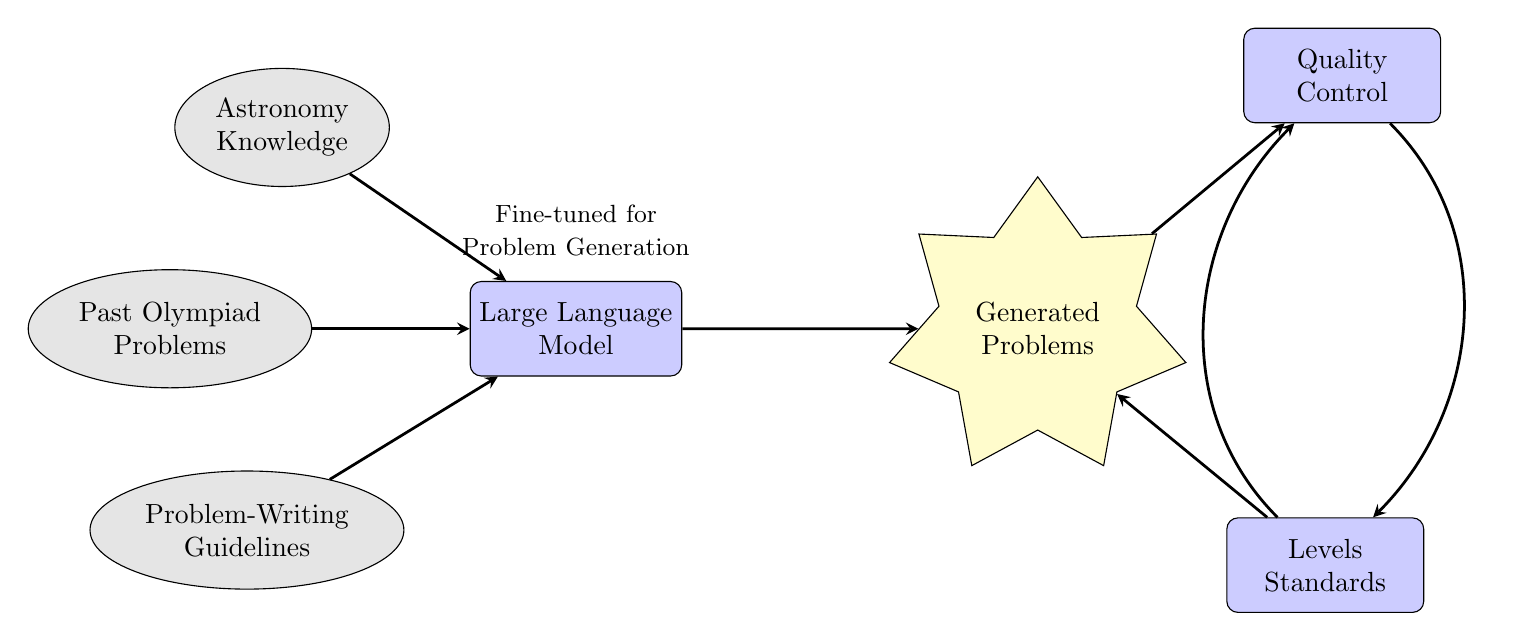
\begin{tikzpicture}[
        node distance=2cm,
        block/.style={rectangle, draw, rounded corners, fill=blue!20,
        minimum width=2.5cm, minimum height=1.2cm, align=center},
        arrow/.style={very thick,->,>=stealth, line width=1pt},
%        arrow/.style={thick,->,>=stealth},
        cloud/.style={draw, ellipse, fill=gray!20, minimum width=2.5cm,
        minimum height=1.5cm, align=center},
        problem/.style={star, star points=7, draw, fill=yellow!20,
        minimum width=1cm, align=center}
    ]

% Main LLM block
        \node[block] (llm) {Large Language\\ Model};

% Input datasets
        \node[cloud, above left=of llm] (astro) {Astronomy\\ Knowledge};
        \node[cloud, left=of llm] (olymp) {Past Olympiad\\ Problems};
        \node[cloud, below left=of llm] (rules) {Problem-Writing\\ Guidelines};

% Output and quality control
        \node[problem, right=3cm of llm] (problems) {Generated\\ Problems};
        \node[block, above right=of problems] (quality) {Quality\\ Control};
        \node[block, below right=of problems] (standards) {Levels\\ Standards};

% Arrows
        \draw[arrow] (astro) -- (llm);
        \draw[arrow] (olymp) -- (llm);
        \draw[arrow] (rules) -- (llm);
        \draw[arrow] (llm) -- (problems);
        \draw[arrow] (problems) -- (quality);
        \draw[arrow] (standards) -- (problems);

% Add some decorative elements
        \node[above=0.2cm of llm, text width=3cm, align=center]
        {\small Fine-tuned for\\ Problem Generation};

% Add circular arrow around problems indicating iteration
        \draw[arrow] (quality) to[out=-45,in=45] (standards);
        \draw[arrow] (standards) to[out=135,in=-135] (quality);

    \end{tikzpicture}
\end{document}